\beginsong{Die Regenfrau}[wuw={tejo (Walter Scherf), 1953}, bo={60}, index={Der Nebel dämpft das Morgenlicht}]

\markboth{\songtitle}{\songtitle}

\beginverse
\endverse

\centering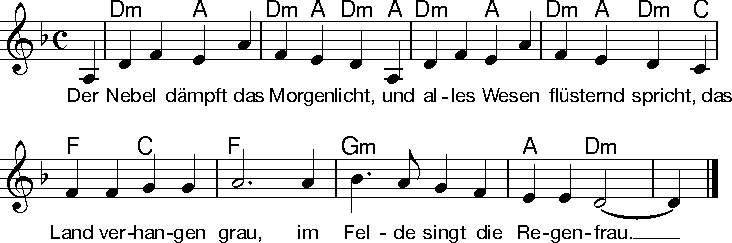
\includegraphics[width=1\textwidth]{Noten/Lied026.pdf}	

\beginverse
Der \[Dm]Weg ist \[A]lang, der \[Dm]Weg \[A]ist \[Dm]weit, \[A]wir \[Dm]wandern \[A]tief am \[Dm]Grund \[A]der \[Dm]Zeit.
Der \[F]Sommer \[C]ist ver\[F]brannt, ein \[Gm]fahler Rauch weht \[A]durch das \[Dm]Land.
\endverse

\beginverse
Das ^Jahr geht ^aus, der ^Re^gen ^fällt, ^ein ^and'rer ^Herr re^giert ^die ^Welt.
Der ^Wind ist ^nass und ^schwer, das ^Land ertrinkt im ^Regen^meer.
\endverse

\endsong

\beginscripture{}
tejo arbeitete auch als Übersetzer, das bekannteste von ihm übersetzte Werk ist ''Der kleine Hobbit'' von J. R. R. Tolkien.
\endscripture

\begin{intersong}
\end{intersong}